\section{{\bf PLAN}}
What will we do...


\subsection{ASTR 598} 

Copied text from that email, which was copied from our book, to see
how many pages it would take...

\subsubsection{Motivation for Astr 598}

Astronomy and astrophysics are witnessing dramatic increases in data volume 
as detectors, telescopes, and computers become ever more powerful. During the 
last decade, sky surveys across the electromagnetic spectrum have collected 
hundreds of terabytes of astronomical data for hundreds of millions of sources. 
Over the next decade, the data volume will enter the petabyte domain, and provide 
accurate measurements for billions of sources. Astronomy and physics students 
are not traditionally trained to handle such voluminous and complex data sets. 
Furthermore, standard analysis methods employed in astronomy often lag far 
behind rapid progress in statistics and computer science. The main
goal of this course is to contribute to efficient training of next
generations of students to 
handle the fast growing data sets, not only in astronomy, but in other quantitative 
sciences as well. 

This course will be aimed at physical and data-centric math,
statistics, science and engineering students
who have an understanding of the science drivers for analyzing large data sets but 
may not be aware of appropriate statistical techniques for doing so. The course work 
will provide to students a connection between scientific data analysis problems and 
modern statistical methods. We will limit theoretical discussions to the minimum 
required to understand the algorithms and will build the courses upon an 
example-driven compendium of modern statistical and data mining methods, 
together with carefully chosen examples based on real modern data sets, and of 
current astronomical applications that will illustrate each method introduced in the 
book. Discussion of the advanced material will be supported by appropriate (publicly 
available) Python code and data which will enable students to perform exercises, 
evaluate the techniques, and adapt them to their own fields of interest. We chose to 
use Python, a powerful and flexible programming language that is quickly becoming 
a standard in data-intensive sciences (and elsewhere). 

The target audience for our course includes undergraduate students with scientific 
or engineering background, but it is likely that graduate students
would benefit from it too. Familiarity with calculus and other basic mathematical 
techniques will be assumed, but no extensive prior knowledge in statistics will be 
required. 

The course outline: 

\begin{enumerate} 
\item Computational Challenges in data-intensive astronomy and astrophysics
\begin{itemize}
\item  data types and data management systems 
\item  analysis of algorithmic efficiency
\item  types of computational problems and strategies for speeding them up 
\item  data visualization challenges
\item  selection effects and truncated/censored data in astronomical context 
\end{itemize}
\item Searching for structure in astronomical point data
\begin{itemize}
\item  non-parametric density estimation
\item  nearest-neighbor density estimation
\item  parametric density estimation
\item  finding clusters in data 
\item  correlation functions 
\end{itemize} 
\item Dimensionality reduction
\begin{itemize}
\item  principal component analysis in astronomical context
\item  non-negative matrix factorization 
\item  independent component analysis and projection pursuit 
\item  manifold learning
\end{itemize} 
\item Regression and model fitting
\begin{itemize}
\item  regresion for linear models
\item  non-linear regression
\item  kernel and principal component regression
\item  methods for handling heteroscedastic and non-Gaussian errors 
\item  Gaussian processes
\item  overfitting, underfitting and cross-validation
\end{itemize} 
\item Classification 
\begin{itemize}
\item  generative classification methods
\item  discriminative classification method 
\item  evaluation and comparison of classifiers: ROCcurves 
\end{itemize} 
\item Time series analysis in astronomy
\begin{itemize}
\item  main concepts and tools for time series analysis
\item  analysis of periodic time series 
\item  temporally localized signals
\item  analysis of stochastic processes
\end{itemize} 
\end{enumerate} 


We will use textbook {\it ``Statistics, Data Mining, and Machine Learning in Astronomy:
A Practical Python Guide for the Analysis of Survey Data''} (Princeton Series in Modern 
Observational Astronomy, in press) coauthored by the Co-PIs on this prooposal. 



\subsection{Python Packages} 


\begin{figure*}[!t]
\vskip -1.8in
\includegraphics[width=1.02\hsize,clip]{astroML.eps}
\vskip -2.0in
\caption{We will leverage all the modern python tools available in {\it astroML} and
other packages, including a large number of practical data-intensive exercises developed to
support textbook that will be used with the proposed ASTR 598 course.} 
\label{Fig:astroML}
\end{figure*}


We will leverage all the publicly available modern python tools. In particular, seminar work will be 
built around the {\it astroML} package (available from http://www.astroml.org) that was developed 
to support textbook to be used with the proposed ASTR 598 course. {\it astroML} is a python module 
for machine learning and data mining built on {\it numpy}, {\it scipy}, {\it scikit-learn}, and {\it matplotlib}, 
and distributed under the 3-clause BSD license. It contains a growing library of statistical and machine 
learning routines for analyzing astronomical data in python, loaders for several open astronomical datasets, 
and a large suite of examples of analyzing and visualizing astronomical datasets (there are close to two 
hundred examples of machine learning and visualization in the code library that supports the textbook 
alone). In addition to  {\it astroML} package, we will expose students to several other popular and widely
used toolkits (e.g. PyMC for Markov chain Monte Carlo methods, and HealPy for spherical coordinates 
and spherical harmonic transformations). 

As an example of methods and exercises available in  {\it astroML}, we single out methods 
for reducing data dimensionality. Many astronomical analyses must address the question of the 
complexity as well as size of the data set. Dimensionality reduction methods address the
complexity issue  by finding the directions within a multivariate data set that contain most 
of the information. Classical approaches for identifying the principal dimensions include
principal component analysis (PCA), independent component analysis (ICA), and non-negative 
matrix factorization (NMF). These methods are implemented in   {\it astroML}, with a user-friendly 
interface and adequate documentation (see Figure~\ref{Fig:astroML}). Furthermore, {\it astroML} also 
includes easy-to-use code to automatically access and download spectra collected by the Sloan Digital 
Sky Survey (currently a ``gold standard'' for modern astronomical surveys and big data sets; see sdss.org). 
Therefore, an undergraduate student will not only be exposed to modern statistical methods
and a cutting-edge astronomical data set, but will be empowered to actually apply these methods 
to a real complex and massive data set.  The result of this exercise is shown in Figure~\ref{Fig:astroML2}. 
With such a positive experience, it is very likely that such a student would not have difficulties applying 
the same methods and tools later to potentially unrelated problems.  


\begin{figure*}[!t]
\vskip -1.8in
\includegraphics[width=1.02\hsize,clip]{astroML2.eps}
\vskip -2.0in
\caption{An example of sophisticated tools available in {\it astroML} and exercises that will be
used in practical seminar work. The figure shows a comparison of the decomposition of SDSS 
spectra using PCA (left panel), ICA (middle panel) and NMF (right panel). The rank of the component
increases from top to bottom. For the ICA and PCA the first component is the mean spectrum (NMF 
does not require mean subtraction). All of these techniques isolate a common set of spectral features 
(identifying features associated with the continuum and line emission). The ordering of the spectral 
components is technique dependent.} 
\label{Fig:astroML2}
\end{figure*}


\subsection{Workshop} 


At the last meeting, we assumed a 3-day workshop for about 30 faculty from other institutions
of higher learning who would want to emulate our program. Further assuming \$20/day/person
for lunch and coffee, and \$75/person for conference dinner, \$1,500 for the workshop venue,
and four grants of \$500 to young faculty and postdocs, we need about \$7,500 for the workshop. 



\subsection{Budget} 

We assumed a 3-year long project. 

We assumed 2.5 months of summer salary for Marina, and a postdoc. About \$150,000/year. 

We assumed 1 month of summer salary for both \v{Z}I and Andy to demonstrate seriousness,
and a graduate student. About \$100,000/year. 

All together, about \$750,000 for 3 years. If this is above the limit, perhaps we could 
descope faculty to only the first two years? 



